% !TEX root = ../thesis-example.tex
%
\chapter{Synchronisation}
\label{sec:Synchronisation}

\cleanchapterquote{The most important property of a program is whether it accomplishes the intention of its user.}{C.A.R. Hoare}{(British computer scientist, winner of the 1980 Turing Award)}

Synchronisation beschreibt den Datenaustausch zwischen einem Sender und einem Empfänger. Dabei werden die Daten in Blöcke aufgeteilt und in einen Übertragungsrahmen eingepasst. Um die Daten aneinander anzugleichen muss dabei festgestellt werden, welches Endgerät welche Daten besitzt und kontrolliert ob das andere Gerät diese Daten zu seinen besitzen will.

Besitzen beide Endgeräte dieselben Daten, z.B. in unterschiedlichen Versionen, kann definiert werden, wie mit den Änderungen umgegangen wird.\cite[]{WEB:SYNCML:2014}

Durch die Begrenzung des lokalen Gerätespeichers würde ich die Synchronisation auf 2 seperaten Wegen durchführen. Im ersten Teil die Datenbank und als Zweites alle Anhänge, wie z.B. Bilder oder Dokumente. So kann das Problem der Speicherbegrenzung bei Webapps umgangen werden.

\section{Datenbanksynchronisation am Bsp. WebSqlSync}
\label{sec:dbsync}

WebSqlSync ist eine Javascript Bibliothek zur automatischen Synchronisation einer lokalen WebSql Datenbank mit dem Server. Die Synchronisation kann dabei in beide Richtungen erfolgen und arbeitet auf dem Prinzip der inkrementellen Synchronisation, was bedeutet dass nur erforderliche Daten übertragen werden.

WebSqlSync funktioniert auch ohne Internetverbindung. Alle Änderungen der Daten werden dabei verfolgt und mit dem Server abgeglichen, sobald wieder eine Internetverbindung besteht. Es wird auch die Änderung auf mehreren Geräten unterstützt.

Die Unterstützung von webapp und der phonegap app für mobile Betriebssysteme wie z.B. iOS und Android ermöglicht eine einfache Integration ohne den Programmcode anpassen zu müssen.\cite[]{WEB:WEBSQLSYNC:2014}

\cleardoublepage

\textbf{Installation und Initialisierung}

Um WebSqlSync nutzen zu können, muss nur die Datei webSqlSync.js im \ac{HTML} des Projekts hinzugefügt werden.

\lstset{language=html}
\lstinline$<script src="lib/webSqlSync.js" type="application/x-javascript" charset="utf-8"></script>$

Wird die Bibliothek aufgerufen, werden automatisch 2 Datenbanktabellen erstellt, falls diese nicht bereits von einem vorherigen Aufruf existieren. Die erste Tabelle \textbf{\lstinline$new_elem$} speichert alle neuen bzw. geänderten Elemente und die zweite Tabelle \textbf{\lstinline$sync_info$} das Datum der letzten Synchronisation.

Zusätzlich werden sogenannte SQLite Auslöser erstellt, die überwachen ob Änderungen per \textbf{\lstinline$INSERT$} oder \textbf{\lstinline$UPDATE$} an den Tabellen vorgenommen wird. SQLite ist eine einfache Datenbankbibliothek die Befehle der Sprache \ac{SQL} verwendet.

Geänderte Elemente werden somit automatisch in der Tabelle \textbf{\lstinline$new_elem$} eingefügt.

\lstset{language=html}
\begin{lstlisting}
DBSYNC.initSync(
	TABLES_TO_SYNC, webSqlDb, sync_info,
	'http://www.myserver.com', callBackEndInit
);
\end{lstlisting}

Die Tabellen die man mit dem Server synchronisieren möchte, werden in der Funktion \textbf{\lstinline$TABLES_TO_SYNC$} angegeben.

\lstset{language=html}
\begin{lstlisting}
TABLES_TO_SYNC = [
  {tableName : 'table1', idName : 'the_id'},
  {tableName : 'table2'}
  //if idName not specified, it will assume that it's "id"
];
\end{lstlisting}

In der Tabelle \textbf{\lstinline$sync_info$} können alle Informationen gespeichert werden, die der Entwickler als nützlich empfindet. Die Identifikation des Clients wäre eine wichtige Eigenschaft, da Sie mit an den Server gesendet wird. Dafür kann jegliche Information genutzt werden, wie z.B. die Emailadresse, ein Login oder auch eine entsprechende \ac{ID} des genutzten mobilen Endgeräts.

\cleardoublepage

\textbf{Aufruf}

Um die Synchronisation zu starten ruft man die Funktion \textbf{\lstinline$syncNow$} auf. Die Synchronisation kann dabei nach einer freiwählbaren Zeitspanne, oder aber nach einer festgelegten Anzahl von Datenänderungen erfolgen.

\lstset{language=html}
\begin{lstlisting}
DBSYNC.syncNow(callBackSyncProgress, function(result) {
  if (result.syncOK === true) {
    //Synchronized successfully
  }
});
\end{lstlisting}

Bei größeren Datenmengen ist es für den Nutzer hilfreich, wenn man eine Fortschrittsanzeige bekommt. Während der Synchronisation wird dafür bei jedem Einzelschritt die Funktion \textbf{\lstinline$callBackSyncProgress$} aufgerufen.

\lstset{language=html}
\begin{lstlisting}
callBackSyncProgress: function(message, percent, msgKey) {
  $('#uiProgress').html(message+' ('+percent+'%)');
},
\end{lstlisting}

\textbf{Einschränkungen}

Die Bibliothek WebSqlSync hat auch ein paar wenige Einschränkungen. Z.B. wird der \ac{SQL}-Befehl \textbf{\lstinline$DELETE$} nicht unterstützt. Stattdessen sollte das mit einem update an der entsprechenden Stelle umgangen werden.

\section{Dateisynchronisation am Bsp. ownCloud}
\label{sec:datasync}

ownCloud ist eine Open Source Software für die Einrichtung einer unabhängigen Serverseitigen Datenspeicherlösung. Sogenannte Cloudspeicher gibt es mittlerweile sehr viele. Die wohl bekanntesten sind Dropbox, Google Drive und OneDrive. Sie ermöglichen einen einfachen Datenzugriff von überall auf der Welt. Dafür lädt man seine Dateien über eine Internetverbindung auf einen speziellen Datenserver. Leider hat das den großen Nachteil, dass man keine 100 prozentige Sicherheit hat, was mit den eigenen Daten passiert.

Um das zu sicherzustellen bietet ownCloud eine Möglichkeit einen eigenen Cloudserver zu erstellen, auf dem man alles selbst konfigurieren kann. Per Nutzer- und Rechteverwaltung lässt sich wie auf einem normalen Server festlegen, wer was machen kann. 

Dazu werden Backup Lösungen angeboten, so dass jederzeit Sicherungen der Dateien angelegt werden können. Der wohl wichtigste Punkt ist aber die Verschlüsselung der gespeicherten Daten mittels \ac{SSL}, somit können auch unternehmensrelevante Daten gespeichert werden.

Durch die Open Source Lösung, lässt sich zu den bereits vorhandenen Plugins, neue Software entwickeln und den eigenen Bedürfnissen anpassen. Da bereits Apps für die mobilen Betriebssystem zu Verfügung stehen, lassen sich relativ einfach Daten zwischen dem Server und dem Client synchronisieren.

Neben der frei verfügbaren ``Community Edition'' stehen für die volle Unterstützung der ownCloud Entwickler auch eine ``Business'' und eine ``Enterprise Version'' zur Verfügung, welche gegen eine jährliche Gebühr angeboten wird.\cite[]{WEB:OWNCLOUD:2014}

\hspace{2 cm}

\begin{figure}[htb]
	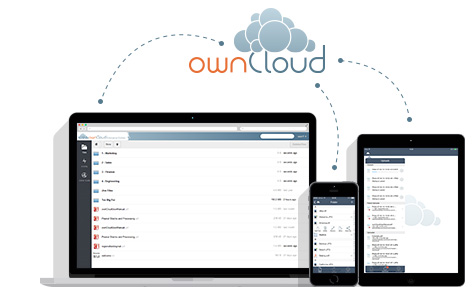
\includegraphics[width=\textwidth]{Bilder/architecture}
	\caption{Architektur ownCloud}
	\label{Datenerfassung}
\end{figure}

\hspace{2 cm}

\textbf{Vorteile Android/iOS App}


\begin{itemize}

	\item SSL- und HTTP-Verbindungen werden automatisch erkannt, so dass eine einfache und gesicherte Verbindung zu dem Server möglich wird.\cite[]{WEB:OWNCLOUD:2014}

	\item Dateien und Ordner auf dem Server können neu angelegt, durchsucht, umbenannt und gelöscht werden, je nachdem wie die Rechte an den Nutzer vergeben sind.\cite[]{WEB:OWNCLOUD:2014}

	\item Durch das Anlegen von Favoriten lassen sich Daten wie Dokumente, Bilder und Videos automatisch mit dem Server synchronisieren.\cite[]{WEB:OWNCLOUD:2014}

\end{itemize}

\hspace{2 cm}

\begin{figure}[htb]
	\begin{tabular}{l r}
		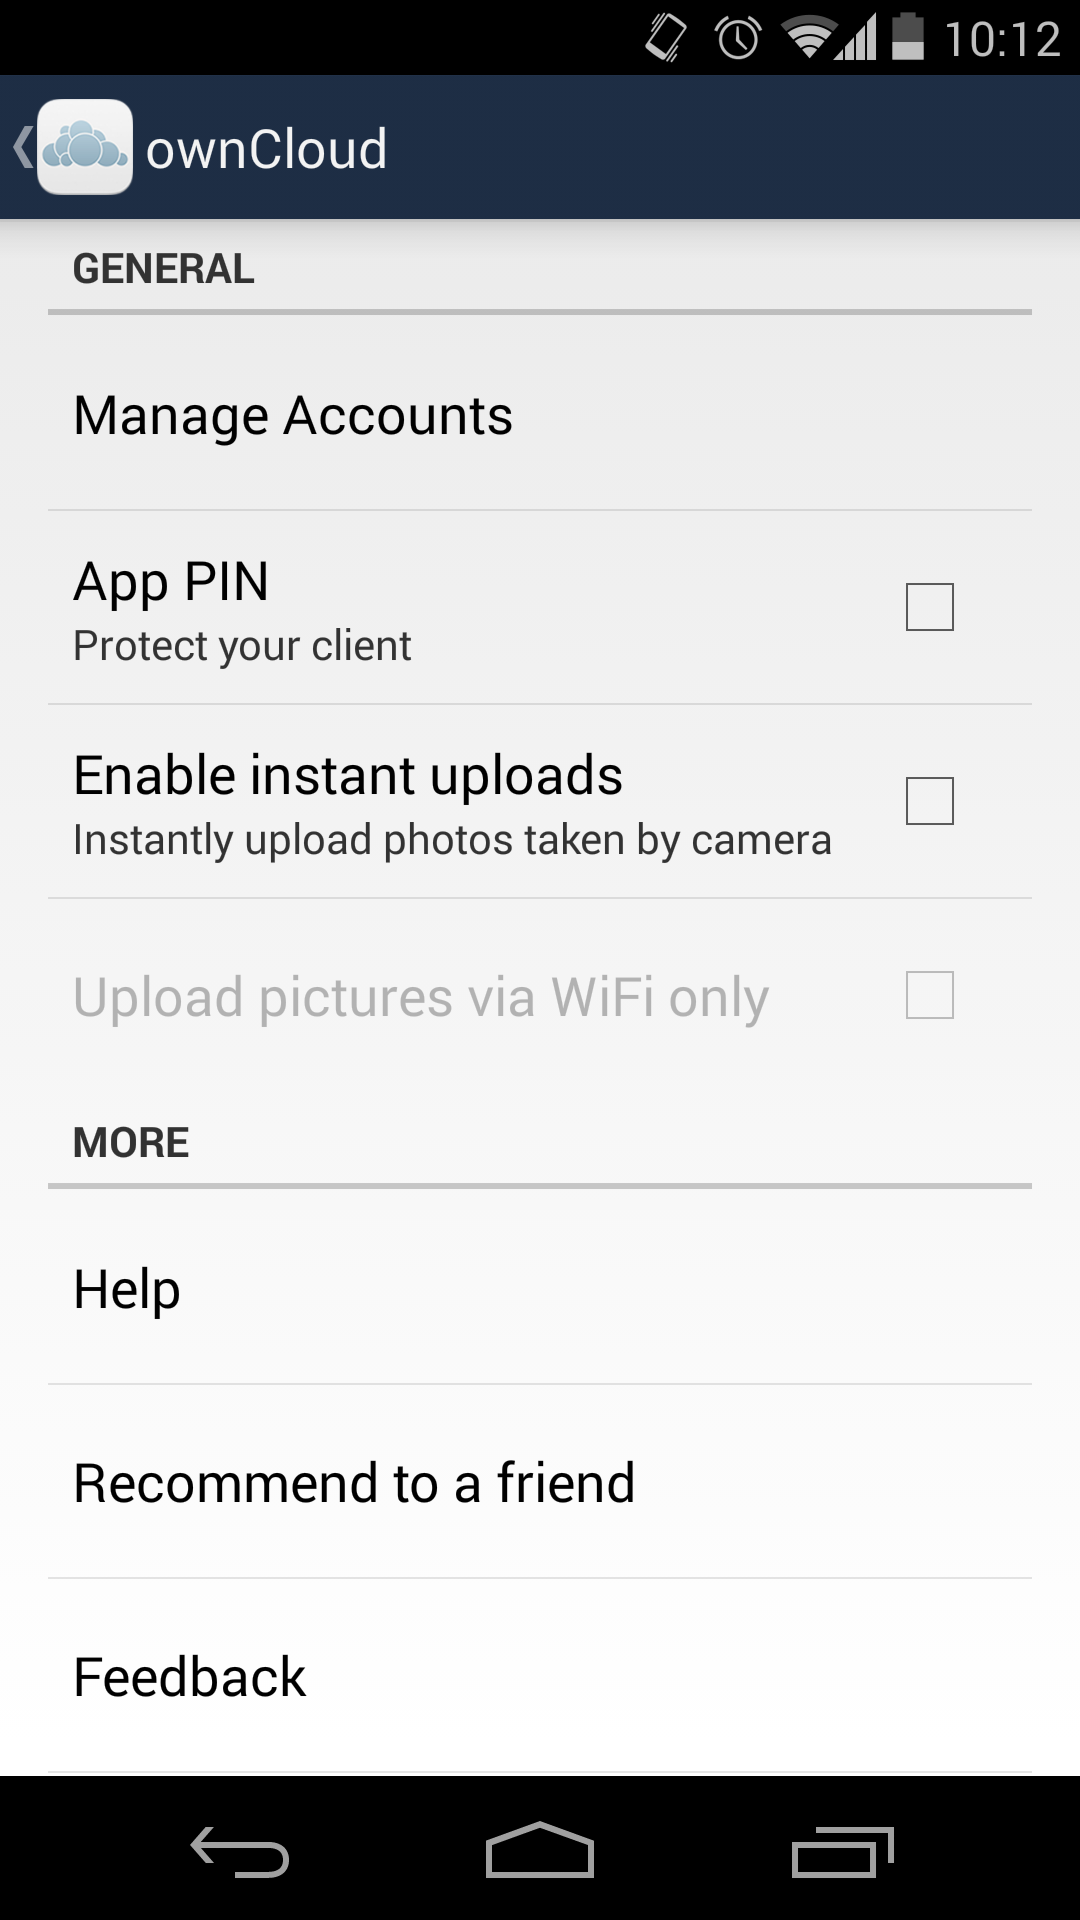
\includegraphics[width=0.49\textwidth]{Bilder/ownCloud-mobile1}
		&
		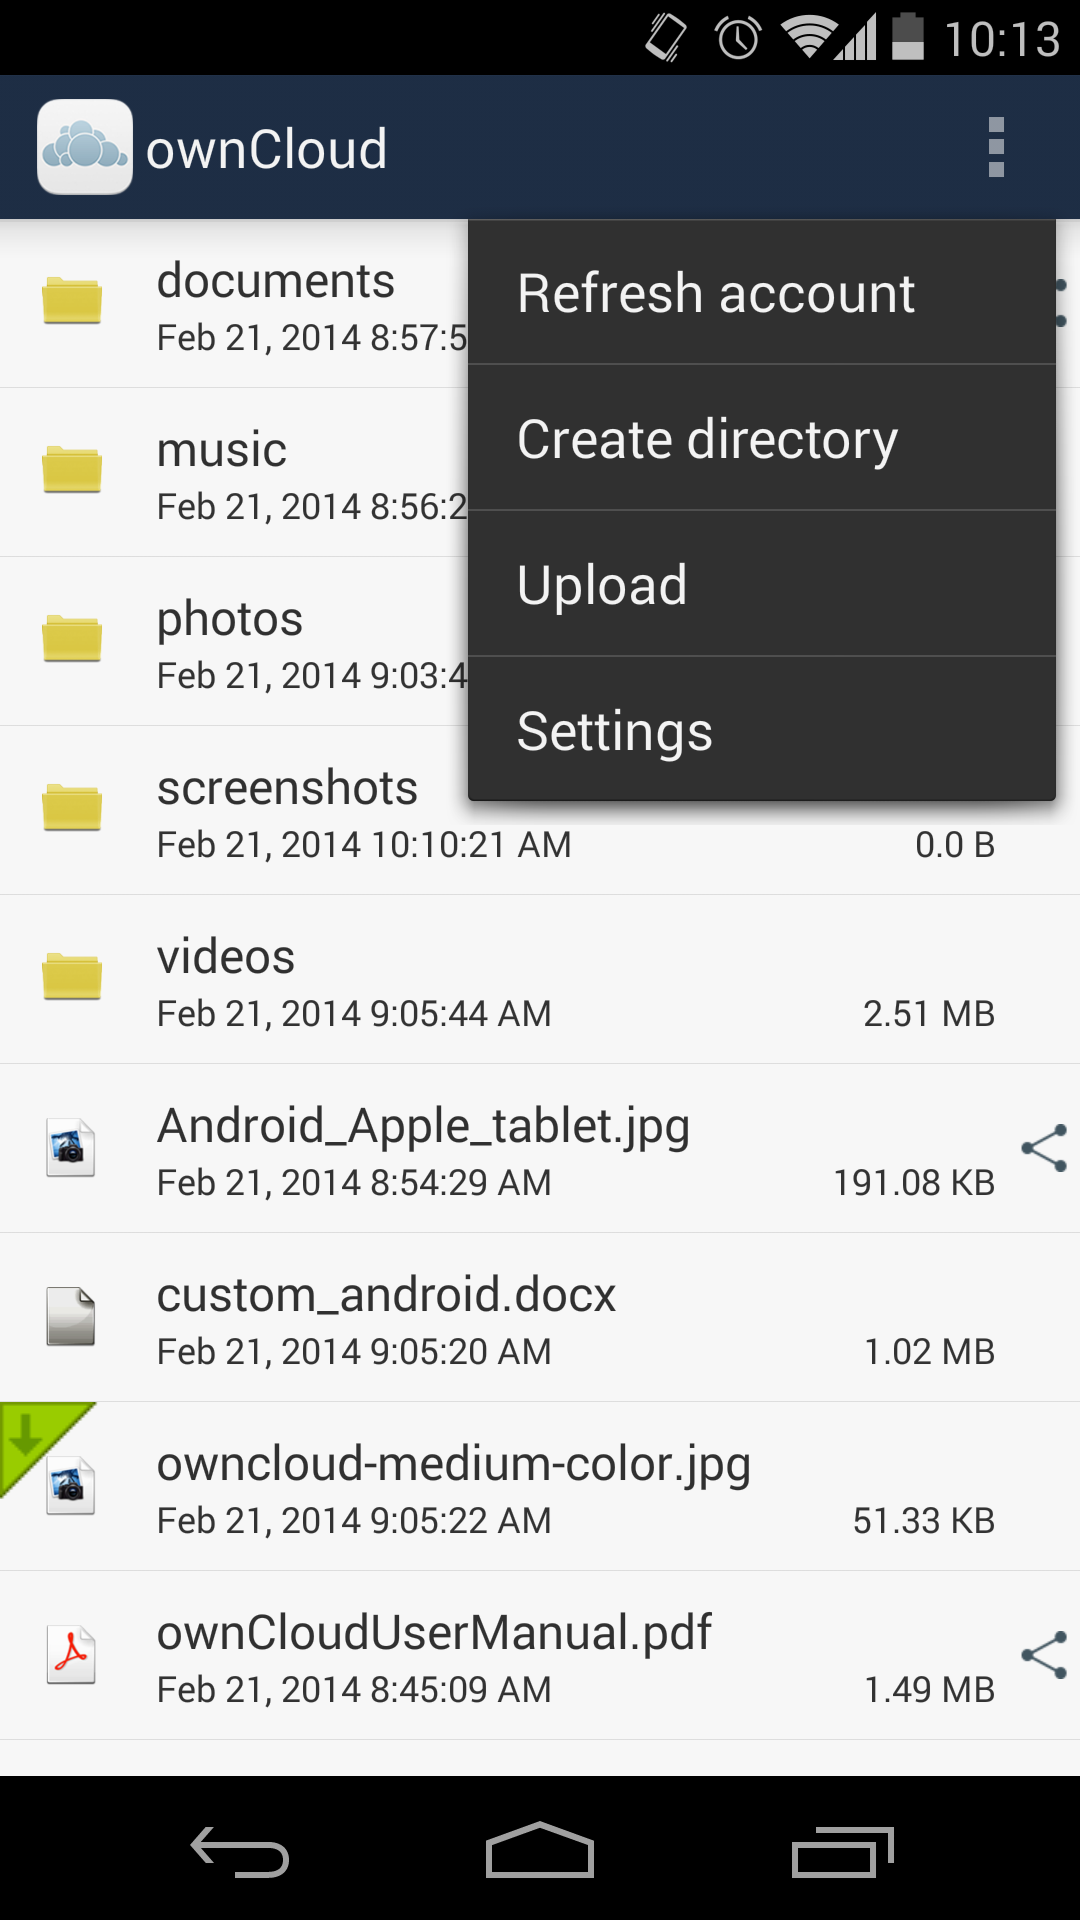
\includegraphics[width=0.49\textwidth]{Bilder/ownCloud-mobile2}
	\end{tabular}
	\caption{ownCloud App}
	\label{Websitemobil}
\end{figure}

\cleardoublepage

